\setcounter{chapter}{26}
\chapter{Boundary Conditions for Electric Fields}\label{chap27}

Under static condition, as all charges lie on the outer surface of the conductor, the $\overrightarrow{E}$ and $\overrightarrow{D}$ are zero within the conductor.

\section{Boundary conditions at the conductor-dielectric\break interface}
\begin{figure}[H]
\centering
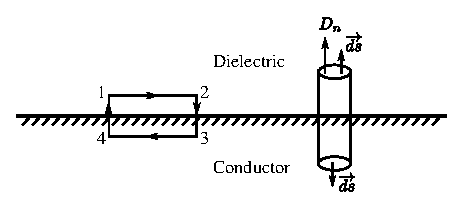
\includegraphics[scale=1.1]{images/fig1.eps}
\caption{Conductor-dielectric interface}\label{chap27-fig1}
\end{figure}

We know that static electric field is a conservative field. 
$$
\text{i.e.,}\qquad \oint \overrightarrow{E} \bigdot \overrightarrow{dL} = 0
$$
Consider a closed rectangular path 12341 shown in Fig.~????
\begin{equation*}
\oint \overrightarrow{E} \bigdot \overrightarrow{dL} = \int\limits_{1}^{2} \overrightarrow{E} \bigdot \overrightarrow{dL} + \int\limits_{2}^{3} \overrightarrow{E} \bigdot \overrightarrow{dL} + \int\limits_{3}^{4} \overrightarrow{E} \bigdot \overrightarrow{dL} + \int\limits_{4}^{5} \overrightarrow{E} \bigdot \overrightarrow{dL} = 0\label{chap27-eq1}
\end{equation*}

In Eqn.~\eqref{chap27-eq1}, the 3$^{\text{rd}}$ integral is zero because the path 3 to 4 is within the conductor where $\overrightarrow{E}$ is zero. If the path lengths 2 to 3 and 4 to 1 approaches zero (i.e., across boundary), the 2$^{\text{nd}}$ and 4$^{\text{th}}$ integral, in Eqn.~\eqref{chap27-eq2} are zero.
\begin{equation*}
\therefore\quad \text{We get } \ \int\limits_{1}^{2} \overrightarrow{E} \bigdot \overrightarrow{dL} = \int E_{t}dL = 0\label{chap27-eq2}
\end{equation*}

Where $E_{t}$ is the tangential component of $\overrightarrow{E}$ at the surface of the dielectric. 

From Eqn.~\label{chap27-eq2}, we get 
$$
 E_{t} = 0\quad \text{\&}\quad D_{t} = 0
$$
Now consider a Gaussian right circular cylinder placed across the boundary as shown in Fig-. From Gauss's law, 
$$
\oint \overrightarrow{D} \bigdot \overrightarrow{ds} = Q_{\text{enclosed}}.
$$
\begin{equation*}
\int\limits_{\text{top}} \overrightarrow{D} \bigdot \overrightarrow{ds} + \int\limits_{\text{bottom}} \overrightarrow{D} \bigdot \overrightarrow{ds} + \int\limits_{\text{side}} \overrightarrow{D} \bigdot \overrightarrow{ds} = \int\limits_{s} P_{s}ds\label{chap27-eq3}
\end{equation*}

In Eqn.~\eqref{chap27-eq3}, the 2$^{\text{nd}}$ integral is zero because the bottom of the cylinder is within the conductor where $\overrightarrow{D}$ and $\overrightarrow{E}$ are zero. The 3$^{\text{rd}}$ integral is zero because $D_{t} = 0$. 
\begin{align*}
\therefore \ & \oint\limits_{\text{top}} \overrightarrow{D} \bigdot \overrightarrow{ds} = \int\limits_{\text{top}} D_{n}ds = \int\limits_{s} \rho_{s}ds\\
\therefore \ & D_{n} = \rho_{s} ~\&~ E_{n} = \dfrac{\rho_{s}}{\epsilon}
\end{align*}

\section{Boundary conditions at the dielectric-dielectric\break interface}\label{chap27-sec2}
\begin{figure}[H]
\centering
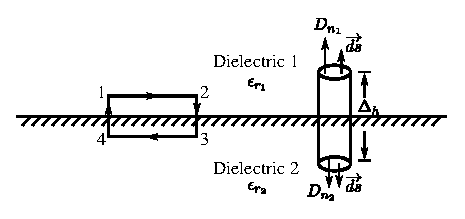
\includegraphics[scale=1.1]{images/fig2.eps}
\caption{Dielectric-dielectric interface}\label{chap27-fig2}
\end{figure}


Consider a dielectric - dielectric interface as shown in Fig.~\ref{chap27-fig2}

Applying Eqn.~\eqref{chap27-eq4} to the closed path 12341,
\begin{equation*}
\int\limits_{1}^{2} \overrightarrow{E} \bigdot \overrightarrow{dL} + \int\limits_{2}^{3} \overrightarrow{E} \bigdot \overrightarrow{dL} + \int\limits_{3}^{4} \overrightarrow{E} \bigdot \overrightarrow{dL} + \int\limits_{4}^{1} \overrightarrow{E} \bigdot \overrightarrow{dL} = 0\label{chap27-eq4}
\end{equation*}

In Eqn.~\eqref{chap27-eq4}, if the path lengths 2 to 3 and 4 to 1 approaches zero (i.e.., across boundary), the 2$^{\text{nd}}$ and 4$^{\text{th}}$ integrals are zero. 
\begin{align*}
\therefore\quad  &\int\limits_{1}^{2} \overrightarrow{E} \bigdot \overrightarrow{dL} + \int\limits_{3}^{4} \overrightarrow{E} \bigdot \overrightarrow{dL} = 0\\
 & \int E_{t_{1}}dL - \int E_{t_{2}}dL  = 0\\
 & \int \left(E_{t_{1}} - E_{t_{2}}\right)dL  = 0\\
 & E_{t_{1}} - E_{t_{2}} = 0
\end{align*} 
$$
\therefore\quad E_{t_{1}} = E_{t_{2}} \quad\text{\&}\quad \dfrac{D_{t_{1}}}{\varepsilon_{r_{1}}} = \dfrac{Dt_{2}}{\varepsilon_{r_{2}}}
$$
Therefore across dielectric-dielectric interface 
tangential component of $\overrightarrow{E}$ is continuous cylindrical. 

Applying Eqn~.\eqref{???}, to the Gaussian surface, 
\begin{equation*}
\int\limits_{\text{top}} \overrightarrow{D} \bigdot \overrightarrow{ds} + \int\limits_{\text{bottom}} \overrightarrow{D} \bigdot \overrightarrow{ds} + \int\limits_{\text{side}} \overrightarrow{D} \bigdot \overrightarrow{ds} = \int\limits_{s} P_{s}ds\label{chap27-eq27.5}
\end{equation*}

In Eqn.~\eqref{????}, as $\Delta h$ approaches zero (i.e., across boundary) the 3$^{\text{rd}}$ integral in Eqn.~???? is zero. The RHS of Eqn.~???? is zero because is dielectric $\rho_{s} = 0$.
\begin{align*}
& \int\limits_{\text{top}} \overrightarrow{D} \bigdot \overrightarrow{ds} + \int\limits_{\text{bottom}} \overrightarrow{D} \bigdot \overrightarrow{ds} = 0\\
& \int Dn_{1}ds - \int Dn_{2}ds  = 0\\
& \int (D_{n_{1}} - D_{n_{2}})ds = 0\\
& D_{n_{1}} - D_{n_{2}}  = 0
\end{align*}
$$
\therefore\quad  D_{n_{1}} = D_{n_{2}}  \quad\text{\&}\quad \varepsilon_{r_{1}}E_{n_{1}} = \varepsilon_{r_{2}}E_{n_{2}}. 
$$
Therefore across dielectric-dielectric interface normal component of $\overrightarrow{D}$ is continuous. 

\begin{problem}
Given that $\overrightarrow{E}_{1} = 2\overrightarrow{a}_{x} - 3\overrightarrow{a}_{y} + 5\overrightarrow{a}_{z}$ across dielectric-dielectric interface shown in Fig.~\ref{chap27-fig3}. Find $\overrightarrow{E}_{2}, \overrightarrow{D}_{1}, \overrightarrow{D}_{2}$ and the angles $\theta_{1}$ and $\theta_{2}$. 
\begin{figure}[H]
\centering
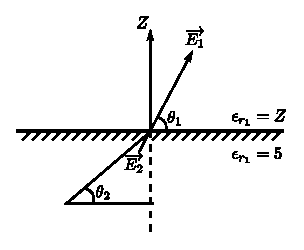
\includegraphics[scale=1.1]{images/fig3.eps}\label{chap27-fig3}
\end{figure}
\end{problem}

\begin{solution}
$\overrightarrow{a}_{x}$ and $\overrightarrow{a}_{y}$ are tangential \& $\overrightarrow{a}_{2}$ is normal to the interface

Given : $\overrightarrow{E}_{1} = 2\overrightarrow{a}_{x} - 3\overrightarrow{a}_{y} + 5\overrightarrow{a}_{z}$
$$
\therefore\quad \overrightarrow{D}_{1} = \varepsilon_{0}\varepsilon_{r_{1}} = 4\varepsilon_{0}\overrightarrow{a}_{x} - 6\varepsilon_{0}\overrightarrow{a}_{y} + 10\varepsilon_{0}\overrightarrow{a}_{z}
$$
From Eqns. ????? \& ?????
\begin{align*}
\overrightarrow{E}_{2} & = 2\overrightarrow{a}_{x} - 3\overrightarrow{a}_{y} + \left(\dfrac{2}{5}\right) 5\overrightarrow{a}_{z}\\
\therefore\quad \overrightarrow{E}_{2} & = 2\overrightarrow{a}_{x} - 3\overrightarrow{a}_{y} + 2\overrightarrow{a}_{z}\\
\overrightarrow{D}_{2} & = \left(\dfrac{5}{2}\right) + \varepsilon_{0}\overrightarrow{a}_{x} - \left(\dfrac{5}{2}\right) 6\varepsilon_{0}\overrightarrow{a}_{y} + 10\varepsilon_{0}\overrightarrow{a}_{z}\\
\therefore\quad \overrightarrow{D}_{2} & = 10\varepsilon_{0}\overrightarrow{a}_{x} - 15\varepsilon_{0}\overrightarrow{a}_{y} + 10\varepsilon_{0}\overrightarrow{a}_{z}
\end{align*}

From Fig.~????
\begin{align*}
E_{z_{1}} & = \overrightarrow{E}_{1} \bigdot \overrightarrow{a}_{z} = E_{1} \cos (90 - \theta_{1})\\
&\quad 5 = \sqrt{2^{2} + 3^{2} + 5^{2}} \sin \theta_{1}\\
&\quad \theta_{1} = 54.2^{\circ}\\[0.3cm]
E_{z_{2}} & = \overrightarrow{E}_{2} \bigdot \overrightarrow{a}_{z} = E_{2} \cos (90 - \theta_{2})\\
&\quad 2 = \sqrt{2^{2} + 3^{2} + 2^{2}} \sin \theta_{2}\\
&\quad \theta_{2} = 29.0^{\circ}
\end{align*}
\end{solution}

\begin{problem}
At the boundary between given ($\varepsilon_{r} = 4$) and air, the lines of electric field makes an angle of $40^{\circ}$ with normal to the boundary. If the electric flux density in air is $0.25 \mu$ c/m$^{2}$, determine the orientation and magnitude of electric flux density in glass. 

\hfill [VTU : Jan 2005, Aug 2001]
\end{problem}

\begin{solution}
~

\begin{figure}[H]
\centering
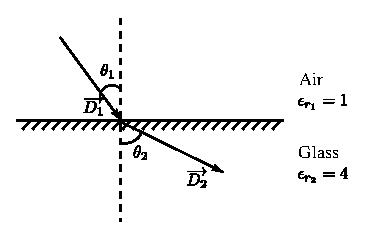
\includegraphics[scale=1.1]{images/fig4.eps}\label{chap27-fig4}
\end{figure}

For dielectric-dielectric interface,
\begin{align*}
D_{t_{1}} & = \dfrac{\varepsilon_{r_{1}}}{\varepsilon_{r_{2}}} \bigdot D_{t_{2}}\\
D_{1} \sin \theta_{1} & = \dfrac{1}{4} D_{2} \bigdot \sin \theta_{2}\\
D_{n_{1}} & = D_{n_{2}}\\
D_{1} \cos \theta_{1} & = D_{2} \cos \theta_{2}\\
\therefore\quad \tan \theta_{1} & = \dfrac{1}{4} \tan \theta_{2}\\
\tan 40 & = \dfrac{1}{4} \tan \theta_{2}\\
\therefore\quad \theta_{2} & = 73.41^{\circ}
\end{align*}

Given that $D_{1} = 0.25\mu$ c/m$^{2}$,

From: Eqn.~???, 
\begin{gather*}
0.25\times 10^{-16} \times \cos 40 = D_{2} \cos 73.41\\
\therefore\quad D_{2} = 0.67\mu \text{c/m}^{2}
\end{gather*}
\end{solution}

\begin{problem}
An electric field strength 1.2 V/m is entering a dielectric medium of $\epsilon_{r} = 4$ from air. The orientation of the electric field in air is $65^{\circ}$ w.r.t the boundary. Determine the orientation and the strength of the electric field in the dielectric medium. 
\end{problem}

\begin{solution}
~

\begin{figure}[H]
\centering
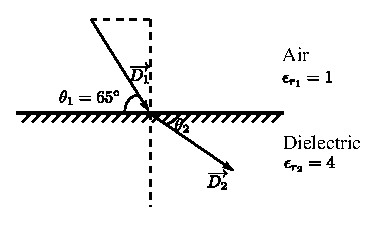
\includegraphics[scale=1.1]{images/fig5.eps}\label{chap27-fig5}
\end{figure}

Across dielectric-dielectric boundary, 
\begin{align*}
E_{t_{1}} & = E_{t_{2}}\\
E_{1} \cos \theta_{1} & = E_{2} \cos \theta_{2}\\
\varepsilon_{r_{1}}E_{n_{1}} & = \varepsilon_{r_{2}}E_{n_{2}}\\
E_{n_{1}} & = \dfrac{\varepsilon_{r_{2}}}{\varepsilon_{r_{1}}} E_{n_{2}}\\
E_{1} \sin \theta_{1} & = \dfrac{\varepsilon_{r_{2}}}{\varepsilon_{1}} E_{2} \sin \theta_{2}\\
\therefore\quad \tan \theta_{1} & = \dfrac{\varepsilon_{r_{2}}}{\varepsilon_{1}} \tan \theta_{2}\\
\tan 65 & = \dfrac{4}{1} \tan \theta_{2}\\
\therefore\quad \theta_{2} & = 28.2^{\circ}
\end{align*}

Given that $E_{1} = 1.2 Vm^{-1}$

From 
\begin{align*}
1.2\cos 65 & = E_{2} \cos 28.2\\
\therefore\quad E_{2} & = 0.575 V/m
\end{align*}
\end{solution}

\begin{problem}
In region $1 ; (z < 0m)$ (free space) where $D_{1} = 5\overrightarrow{a}_{y} + 7\overrightarrow{a}_{z} \text{c/m}^{2}$; region $2 ; (0 < z < 1m)$ has $\epsilon_{r_{2}} = 2.5$ and region $3 ; (z > 1m)$ has $\epsilon_{r_{3}} = 3.0$

Find $E_{1}, D_{2}, E_{2}, D_{3}, E_{3}$ and $\theta_{3}$
\end{problem}

\begin{solution}
~

\begin{figure}[H]
\centering
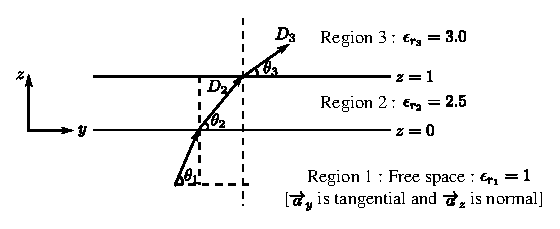
\includegraphics[scale=1.1]{images/fig6.eps}\label{chap27-fig6}
\end{figure}

Given:
\begin{align*}
\overrightarrow{D}_{1} & = 5\overrightarrow{a}_{y} + 7\overrightarrow{a}_{z}\\
\overrightarrow{E}_{1} & = \dfrac{\overrightarrow{D}_{1}}{\varepsilon_{0}} = \dfrac{1}{\varepsilon_{0}} [5\overrightarrow{a}_{y} + 7\overrightarrow{a}_{z}]\\
D_{2} & = \left(\dfrac{2.5}{1}\right) 5\overrightarrow{a}_{y} + 7\overrightarrow{a}_{z} = 12.5\overrightarrow{a}_{y} + 7\overrightarrow{a}_{z}\\
\overrightarrow{E}_{2} & = \dfrac{1}{\varepsilon_{0}\varepsilon_{r_{2}}} \overrightarrow{D}_{2} = \dfrac{1}{\varepsilon_{0}} \left[5\overrightarrow{a}_{y} + \dfrac{7}{2.5} \overrightarrow{a}_{z}\right]\\
\overrightarrow{D}_{3} & = \left(\dfrac{3}{2.5}\right) 12.5\overrightarrow{a}_{y} + 7\overrightarrow{a}_{z} = 15\overrightarrow{a}_{y} + 7\overrightarrow{a}_{z}\\
\overrightarrow{E}_{2} & = \dfrac{1}{\varepsilon_{0}\varepsilon_{r_{3}}} \overrightarrow{D}_{3} = \dfrac{1}{\varepsilon_{0}} \left[5\overrightarrow{a}_{y} + \dfrac{7}{3} \overrightarrow{a}_{z}\right]
\end{align*}

From Fig.~: 
\begin{align*}
D_{z_{3}} & = \overrightarrow{D}_{3} \bigdot \overrightarrow{a}_{z} = D_{3} \cos (90 - \theta_{3})\\
7 & = \sqrt{15^{2} + 7^{2}} \sin \theta_{3}\\
\therefore \theta_{3} & = 25.02^{\circ}
\end{align*}
\end{solution}

\newpage

\begin{itemize}
\item[(a)] Thus current density,
$$
\mathbf{J}=\dfrac{K}{\rho} \ \mathbf{a}_{\rho}=\dfrac{31.4658}{\rho} \ \mathbf{a}_{\rho}A/m^{2}
$$
The electric field intensity in region $2<\rho<3$, 
$$
\mathbf{E}_{1}=\dfrac{K}{100\rho} \ \mathbf{a}_{\rho}=\dfrac{31.4658}{100\rho} \ \mathbf{a}_{\rho}=\dfrac{0.3147}{\rho} \ \mathbf{a}_{\rho} V/m
$$
For $3<\rho<6$, the electric field intensity
$$
\mathbf{E}_{2}=\dfrac{K}{25\rho} \ \mathbf{a}_{\rho}=\dfrac{31.4658}{25\rho} \ \mathbf{a}_{\rho}=\dfrac{1.2586}{\rho} \ \mathbf{a}_{\rho}V/m
$$

\item[(b)] At $\rho=2$ cm, the current crossing the cylindrical surface is
\begin{align*}
I &= |\mathbf{J}|\times 2\pi \rho L=\dfrac{31.3658}{\rho}\times 2\pi \rho L\\[-1pt]
  &= 31.3658\times 2\pi\times 0.5=98.80~\text{A}
\end{align*}
The total current is independent to radius of cylinder $\rho$. The potential between the cylinders is $1$ V. Thus the resistance offered by the cylindrical resistance is
$$
 R=\dfrac{V}{I}=\dfrac{1}{98.80}=0.01012\Omega = 10.12~ \text{m}\Omega
$$

\item[(c)] The potential at $\rho=3$ cm is
\begin{align*}
  V &= - \int\limits^{3}_{6}E_{2}.d\rho =- \int\limits^{3}_{6}\dfrac{31.4658}{25\rho}.d\rho\\[-1pt]
&= \dfrac{31.4658}{25}ln~2=0.8724\text{~V}
\end{align*}
\end{itemize}

\setcounter{problem}{15}
\begin{problem}
The cross-section of the transmission line shown in Fig.~6.24 is drawn on a sheet of conducting paper with metallic paint. The sheet resistance is $2500\Omega$ per square and the dimension $a$ is $1$ in. (a) Assuming a result for Prob. $6b$ of $120 pF/m$, what total resistance would be measured between the metallic conductors drawn on the conducting paper? (b) What would the total resistance be if $a=0.6$ cm?
\end{problem}

Given the metallic paint on the sheet of paper shown in Fig.~6.24. The resistance of sheet is 2500 per square, dimension $a=1$ inch.
\begin{itemize}
\begin{minipage}[t]{5cm}
\item[(a)] The permittivity is $\epsilon_{R}=1.6$. The calculated capacitance is $120$ pF/m. Let the thickness of paper be $t$. The total capacitance offered is $C=120t$ pF. The current is flowing from inner rim to outer rim in a non-uniform fashion.

The product of resistance and capacitance of a similar geometry is
$$
 RC=\dfrac{d}{\sigma S}\times \dfrac{\epsilon S}{d}=\dfrac{\epsilon_{0}\epsilon_{R}}{\sigma}
$$
\end{minipage}
\begin{minipage}[t]{5.2cm}
~
\vskip -.7cm
\begin{figure}[H]
\centering
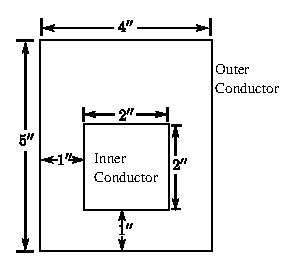
\includegraphics[scale=.9]{images/new-1.eps}
\caption{Metallic paint on the sheet of paper-conduction from inner conductor to outer conductor}
\end{figure}
\end{minipage}

\itemsep=0pt
This gives
$$
 R=\dfrac{1.6\times 8.85}{120 t\sigma}
$$
But the resistance of sheet is 2500 per square dimension $a=1$ inch.
$$
 R_{S}=\dfrac{1}{\sigma\times t}=2500\Omega \Rightarrow \sigma\times t=\dfrac{1}{2500}
$$
Thus the resistance is
$$
 R=\dfrac{1.6\times 8.85}{120 t\sigma}=\dfrac{1.6\times 8.85\times 2500}{120}=295 \Omega
$$

\item[(b)] If $a=0.6$ cm, the resistance of sheet per square inch does not vary by changing the square size, because
$$
 R_{S}=\dfrac{1}{\sigma\times t}=2500\Omega \Rightarrow \sigma\times t=\dfrac{1}{2500}
$$
Thus the resistance is again
$$
 R=\dfrac{1.6\times 8.85}{120 t\sigma}=\dfrac{1.6\times 8.85\times 2500}{120}=295\Omega
$$
\end{itemize}

\begin{problem}
The cross-section of a coaxial transmission line is drawn on a sheet of conducting paper using the dimensions $a=0.5$ in and $b=3$ in. Silver paint is used for the two conducting surfaces. If a resistance of $1000\Omega$ is measured between conductors: (a) What is the resistance per square of the paper? (b) If the conducting layer on the paper is $0.008$ in thick, what is the conductivity of the resistive coating?
\end{problem}

\noindent
Dimension of coaxial line $a=0.5$ in and $b=3$ in. A silver paint is used for the two conducting surfaces.
\begin{itemize}
\itemsep=0pt
\item[(a)] Here resistance between the conductor is $1000\Omega$.

Let the thickness of paint be $t$. The capacitance is
\begin{align*}
C &= \dfrac{2\pi \epsilon_{0}}{ln(b/a)}\times t=\dfrac{2\times \pi \times 8.85}{ln(3/0.5)}\times t=31.09\times t \ \text{pF}\\
\text{But}\qquad RC &= \dfrac{\epsilon_{0}}{\sigma}
\end{align*}
The resistance is
\begin{align*}
R &= \dfrac{\epsilon_{0}}{\sigma C}=\dfrac{8.85 ln (6)}{2\pi\times 8.85\sigma t}=1000\\
\Rightarrow\qquad \sigma t &= \dfrac{ln(6)}{2\pi \times 1000}=2.83\times 10^{-4}
\end{align*}
But the resistance of sheet per square of the paper is
$$
R_{S}=\dfrac{1}{\sigma\times t}=\dfrac{1}{2.83\times 10^{-1}}=3504.94\Omega
$$

\item[(b)] The conducting layer of the coating is $0.008$ in $=0.008\times 0.0254$ m thick. The conductivity of resistive coating is
\begin{align*}
\dfrac{1}{\sigma\times t} &= 3504.94\Omega\\
\text{or}\qquad \sigma &= \dfrac{1}{3504.94\times t}=\dfrac{1}{3504.94\times 0.008\times 0.0254}=1.404  \mho/m
\end{align*}

\end{itemize}


\label{27end}

